\documentclass[journal]{IEEEtran}

\usepackage{amsmath,amssymb,amsfonts}
\usepackage{booktabs}
\usepackage{array}
\usepackage{multirow}
\usepackage{cite}
\usepackage{url}
\usepackage{xcolor}
\usepackage{listings}
\usepackage{balance}
\usepackage{pgfplots}
\pgfplotsset{compat=1.18}
\usepackage{needspace}

\lstdefinelanguage{Lean}{
  morekeywords={theorem,def,structure,inductive,where,match,with,if,then,else,let,in,fun,forall,exists,by,have,show,sorry,exact,simp,omega,decide,native_decide,intro,apply,rfl,instance,class,abbrev,noncomputable,example,lemma,Prop,Type,Nat,Fin,List,Bool,true,false,And,Or,Not},
  sensitive=true,
  morecomment=[l]{--},
  morestring=[b]"
}

\lstset{
  language=Lean,
  basicstyle=\ttfamily\footnotesize,
  keywordstyle=\color{blue!55!black}\bfseries,
  commentstyle=\color{green!40!black}\itshape,
  stringstyle=\color{orange!50!black},
  frame=single,
  breaklines=true,
  columns=fullflexible,
  keepspaces=true,
  showstringspaces=false,
  numbers=none,
  xleftmargin=0.5em,
  aboveskip=0.5em,
  belowskip=0.5em,
  escapeinside={(*}{*)},
  literate={·}{{$\cdot$}}1 {←}{{$\leftarrow$}}1 {→}{{$\rightarrow$}}1 {∀}{{$\forall$}}1 {∃}{{$\exists$}}1 {≤}{{$\leq$}}1 {≥}{{$\geq$}}1 {≠}{{$\neq$}}1 {⟨}{{$\langle$}}1 {⟩}{{$\rangle$}}1 {↔}{{$\leftrightarrow$}}1 {∧}{{$\land$}}1 {∨}{{$\lor$}}1 {¬}{{$\lnot$}}1 {λ}{{$\lambda$}}1 {⊢}{{$\vdash$}}1 {∈}{{$\in$}}1
}

\let\origsection\section
\renewcommand{\section}{\needspace{4\baselineskip}\origsection}
\let\origsubsection\subsection
\renewcommand{\subsection}{\needspace{3\baselineskip}\origsubsection}
\clubpenalty=10000
\widowpenalty=10000
\displaywidowpenalty=10000

\begin{document}

\title{From Rules to Nash Equilibria: Formally Verified\\Game-Theoretic Analysis of a Competitive\\Trading Card Game}

\author{Author names withheld for review}

\maketitle

\begin{abstract}
We present a metagame analysis of the competitive Pok\'emon Trading Card Game, formally verified using Lean~4 and real tournament data.
All game-theoretic results (Nash equilibrium, replicator dynamics, bridge alignment) rely on \texttt{native\_decide}, which trusts Lean's compiler rather than its kernel; the trust boundary is detailed in Section~IX.
The artifact spans approximately 30{,}000 lines, 81 files, and 2{,}500 theorems---of which roughly 190 directly verify empirical claims---with no \texttt{sorry}, \texttt{admit}, or custom axioms.
Analyzing Trainer Hill data (January--February 2026, 50+ player events) over 14 archetypes and their full pairwise matchup matrix, we prove a \emph{popularity paradox}: the most played deck (Dragapult, 15.5\% share) has only 46.7\% expected win rate, while Grimmsnarl (5.1\% share) achieves 52.7\%.
A machine-checked Nash equilibrium with six-deck support assigns Dragapult 0\% weight; exhaustive support enumeration over all $2^{14}-1$ subsets confirms this is the unique symmetric Nash equilibrium of the constant-sum symmetrization, and Dragapult is strictly suboptimal against the equilibrium mix by 63.3 permil.
Single-step replicator dynamics on the \emph{full 14-deck game} indicate downward fitness pressure on Dragapult, upward pressure on Grimmsnarl, and strongest extinction pressure on Alakazam.
A 10{,}000-iteration sensitivity analysis confirms qualitative stability: core support decks appear in $>$96\% of resampled equilibria.
The primary contribution is methodological: formal verification transforms qualitative metagame narratives into machine-checkable, reproducible strategic science.
\end{abstract}

\begin{IEEEkeywords}
Formal verification, game theory, trading card games, Nash equilibrium, theorem proving, metagame analysis, replicator dynamics, Lean~4
\end{IEEEkeywords}

%======================================================================
\section{Introduction}
%======================================================================

Tournament outcomes in competitive trading card games (TCGs) are often shaped before round one begins.
The pre-tournament deck-selection problem is naturally modeled as a strategic game where payoffs derive from matchup win rates and the population distribution of opponents.
The Pok\'emon TCG is especially suitable for this analysis: it has a large organized-play ecosystem, clearly defined public rules, and a metagame that evolves quickly enough to produce measurable strategic cycles, yet hidden information and stochastic effects make intuition unreliable even for experienced players.

By encoding game semantics in Lean~4~\cite{moura2021lean} and proving strategic statements directly over exact data representations, we build a proof-carrying metagame analytics pipeline where the verified objects are
(i)~data representation and ingestion,
(ii)~expected-value computations over the field,
(iii)~machine-checked Nash-equilibrium computation and full 14-deck replicator dynamics, and
(iv)~tournament-objective transforms (Bo3, Swiss).

Our empirical foundation is Trainer Hill metagame data~\cite{trainerhill2026,limitless2024} for 50+ player tournaments from January~29 to February~19, 2026.
We model the top 14 archetypes and their full pairwise matchup matrix.
The paper makes four contributions:
(1)~a machine-checked bridge from type-effectiveness rules to empirical matchup outcomes (Section~\ref{subsec:typealignment});
(2)~verified expected-value computations revealing a popularity paradox;
(3)~machine-checked Nash equilibrium and replicator dynamics over the full 14-deck game; and
(4)~verified best-of-three and Swiss-relevant tournament transforms.

While the headline popularity paradox could be computed in a spreadsheet, the formal verification methodology provides three distinct advantages.
First, \textbf{compositional guarantees}: the Nash equilibrium certification checks best-response conditions for all 14 strategies simultaneously, a 196-cell verification that is error-prone by hand.
Second, \textbf{robustness proofs}: the worst-case bounds (Section~\ref{sec:threats}) require symbolic reasoning over parameterized win rates, not just point arithmetic.
Third, \textbf{reproducibility infrastructure}: the proof artifact serves as a machine-checkable specification that can be re-verified against updated tournament data without re-auditing the analysis logic.

The remainder of the paper is organized as follows.
Section~\ref{sec:related} situates the work.
Section~\ref{sec:formalization} presents the Lean model of rules and legality.
Section~\ref{sec:probability} develops probability and resource theory.
Section~\ref{sec:data} details data and measurement.
Section~\ref{sec:paradox} presents the popularity paradox.
Section~\ref{sec:nash} analyzes equilibrium and dynamics.
Section~\ref{sec:tournament} discusses tournament strategy.
Section~\ref{sec:methodology} documents formalization methodology.
Section~\ref{sec:threats} covers validity threats, and Section~\ref{sec:conclusion} concludes.

%======================================================================
\section{Related Work}\label{sec:related}
%======================================================================

\textbf{Formal methods and strategic games.}
Formal reasoning has transformed analysis in several strategic domains, from Shannon's foundational chess analysis~\cite{shannon1950chess,schaefer1978complexity,fraenkel1981chess} to imperfect-information breakthroughs like Cepheus, Libratus, and Pluribus~\cite{bowling2015heads,brown2018superhuman,brown2019pluribus}, and multi-agent systems like AlphaZero and AlphaStar~\cite{silver2018general,vinyals2019alphastar}.
TCGs are harder in a different way: their compositional card interactions and exception-heavy textual semantics increase the risk of silent modeling errors, which a proof assistant mitigates by forcing explicit treatment of definitions and invariants.

\textbf{AI and metagame analysis in card games.}
Prior card-game AI work has emphasized in-game decision quality via Monte Carlo methods~\cite{cowling2012information,ward2009monte,santos2017monte,zhang2017deck} and deckbuilding optimization~\cite{bjorke2017deckbuilding,dockhorn2019hearthstone,kowalski2020summon}.
That line of work is orthogonal to our question: how should a player choose a deck before round one, given a population distribution and matchup matrix?
Our approach fills this gap by treating metagame analysis as theorem proving over empirical constants.

\textbf{Theorem proving for rule systems.}
Lean~4~\cite{moura2021lean} combines expressive dependent types with efficient decision procedures, and large collaborative libraries demonstrate the maturity of this ecosystem~\cite{gonthier2008four,Avigad2007,mathlib2020,hales2017kepler}.
Related work has explored formalization of card-game rule systems in proof assistants~\cite{li2023card}; our work differs by coupling rule formalization to a complete, real matchup matrix and then pushing through equilibrium and dynamics claims.

\textbf{Evolutionary perspectives.}
Replicator dynamics~\cite{smith1973logic,taylor1978evolutionary,weibull1997evolutionary} provide a natural lens for metagame adaptation.
We use evolutionary tools not as informal metaphors but as theorem-backed statements over fixed data: when we claim Dragapult has negative relative fitness, that claim is a machine-checked consequence of the encoded matchup matrix and observed share vector.



%======================================================================
\section{Game Formalization}\label{sec:formalization}
%======================================================================

We formalize the strategic layer of the Pok\'emon TCG in Lean~4, grounded in official rule documents~\cite{ptcg_rules,playpokemon2024rules}.
The formalization encodes game state (\texttt{GameState} with per-player zones, turn ownership, and a finite phase machine), deck legality (a computable checker linked to an inductive specification via \texttt{checkDeckLegal\_iff}), and card-flow invariants (conservation of total card count, bench-size bounds, prize-card accounting).
The complete formalization spans 15 files in the supplementary artifact.

\textbf{Type effectiveness.}
Weakness and resistance are total functions over enumerated types.
The type effectiveness triangle is certified:

\begin{lstlisting}
-- TypeEffectiveness.lean:138
theorem TRIANGLE :
    ∃ A B C : PType,
      weakness A B = true ∧ weakness B C = true ∧ weakness C A = true := by
  exact ⟨PType.grass, PType.fire, PType.water, rfl, rfl, rfl⟩
\end{lstlisting}

\textbf{Card conservation} is verified for high-impact trainer cards.
For Professor's Research, we prove that discarding the hand and drawing seven preserves global card count, preventing subtle bookkeeping bugs from distorting probability estimates:

\begin{lstlisting}
-- CardEffects.lean:149
theorem professorsResearchEffect_preserves_cards
    (p : PlayerState) :
    playerCardCount (professorsResearchEffect p)
      = playerCardCount p := by
  unfold professorsResearchEffect playerCardCount
  simp [List.length_take, List.length_drop,
        List.length_append]
  omega
\end{lstlisting}

\textbf{Rules--empirical integration.}
The deck legality biconditional ensures only tournament-legal configurations enter the analysis, and the type effectiveness formalization provides machine-checked validation that archetype classifications respect the game's underlying strategic structure.
As shown in Section~\ref{subsec:typealignment}, the rules layer generates falsifiable type-advantage predictions that the empirical matrix largely confirms (83\%+ alignment), with explicitly characterized exceptions.
The formalization also future-proofs the framework for counterfactual analysis (e.g., ``what if a card is banned?'') and enables consistency checks between rule-level predictions and empirical matchup data.

\subsection{From Type Rules to Matchup Data}\label{subsec:typealignment}

Each archetype is assigned primary attack and defense types reflecting its main attacker's typing (e.g., Grimmsnarl uses Dark-type attacks; Dragapult is a Psychic-type defender).
These are domain-expert modeling choices formalized in \texttt{ArchetypeAnalysis.lean}; all assignments are explicitly listed and auditable.

\paragraph{Type assignment methodology}
The primary attack/defense type assignments are not formally derived from deck composition or card data.
Each archetype is classified by the type of its main attacker (for offense) and its primary active Pok\'emon (for defense), based on the dominant game-plan of the deck.
For most archetypes these assignments are unambiguous, but multi-type decks like Dragapult Charizard require judgment about which type dominates.
The 83\% alignment rate reported below would change if borderline assignments were revised; we treat these assignments as modeling assumptions within the formal boundary.

\begin{lstlisting}
-- ArchetypeAnalysis.lean
def hasTypeAdvantage (attacker defender : Deck) : Bool :=
  weakness (Deck.primaryDefenseType defender)
           (Deck.primaryAttackType attacker)
\end{lstlisting}

The alignment between rule-level type advantages and empirical outcomes is striking.
Among Dark-type attackers (Grimmsnarl, Mega Absol, N's Zoroark) facing Psychic-type defenders (Dragapult, Gardevoir, Gardevoir Jellicent, Dragapult Charizard, Alakazam), the empirical matchup exceeds 50\% in 13 of 15 pairs.
Grimmsnarl achieves a perfect 5-for-5 against Psychic defenders (56.6\%--59.9\%); Mega Absol mirrors this at 5-for-5.

\begin{lstlisting}
-- ArchetypeAnalysis.lean
theorem grimmsnarl_dark_beats_all_psychic :
    matchupWR .GrimssnarlFroslass .DragapultDusknoir > 500 (*$\wedge$*)
    matchupWR .GrimssnarlFroslass .Gardevoir > 500 (*$\wedge$*)
    matchupWR .GrimssnarlFroslass .GardevoirJellicent > 500 (*$\wedge$*)
    matchupWR .GrimssnarlFroslass .DragapultCharizard > 500 (*$\wedge$*)
    matchupWR .GrimssnarlFroslass .AlakazamDudunsparce > 500
    := by decide
\end{lstlisting}

The two exceptions---both involving N's Zoroark---illustrate that type advantage is necessary but not sufficient: deck-specific interactions modulate the prediction.
Overall, 83\% alignment (15/18 matchups, $p < 0.001$ under binomial null) confirms the consistency is not coincidental.
For context, random type assignments would yield approximately 50\% alignment by symmetry.

This bridge has direct consequences for the popularity paradox.
Dragapult's Psychic typing makes it structurally vulnerable to the 13.1\% of the meta occupied by Dark-type attackers.
Four independently verified facts align: (i)~the \emph{rules} specify Psychic is weak to Dark; (ii)~the \emph{type assignments} classify Dragapult as Psychic-defending; (iii)~the \emph{empirical data} confirms Dark attackers hold positive win rates vs Dragapult; and (iv)~the \emph{population weights} show 13.1\% exploits this disadvantage.
The formal contribution is verifying that these four layers are mutually consistent, not that any one causes the next.

\needspace{12\baselineskip}
\begin{lstlisting}
-- ArchetypeAnalysis.lean
theorem dragapult_type_vulnerability :
    weakness (Deck.primaryDefenseType .DragapultDusknoir)
             .dark = true (*$\wedge$*)
    metaShare .GrimssnarlFroslass
      + metaShare .MegaAbsolBox
      + metaShare .NsZoroark = 131 (*$\wedge$*)
    matchupWR .DragapultDusknoir .GrimssnarlFroslass < 500 (*$\wedge$*)
    matchupWR .DragapultDusknoir .MegaAbsolBox < 500 (*$\wedge$*)
    matchupWR .DragapultDusknoir .NsZoroark < 500 := by
  constructor <;> decide
\end{lstlisting}

\paragraph{Numerical sufficiency}
A stronger theorem (\texttt{dark\_weakness\_sufficient\_for\_suboptimality}) proves that Dark-type weakness \emph{alone} is numerically sufficient to explain Dragapult's sub-50\% fitness: even granting 50\% against every non-Dark opponent, the Dark-type losses drag its population-weighted expected value below 50\%.
Specifically:
\[
  \underbrace{\sum_{j \in \text{Dark}} s_j \cdot w_{\text{Drag},j}}_{\text{verified losses}} + \underbrace{(695 - 131) \times 500}_{\text{best-case non-Dark}} < 500 \times 695.
\]
This is a machine-checked numerical verification over concrete constants: the rules formalization provides numerical evidence that type disadvantage alone accounts for the popularity paradox.

A companion module (\texttt{IntegrationTests.lean}) collects 12 cross-module integration theorems spanning the full infrastructure, including a summary theorem (\texttt{the\_complete\_story}) conjoining 11 cross-module facts into one machine-checked consistency check.

%======================================================================
\section{Probability and Resource Theory}\label{sec:probability}
%======================================================================

Strategic performance in TCGs is constrained by stochastic access (draws, coin flips, prize placement) and deterministic bottlenecks (energy attachment limits, phase restrictions).
Our Lean development captures both dimensions using exact arithmetic over rational values.
Opening-hand consistency follows hypergeometric structure: the canonical ``four-of in opening seven'' probability is approximately 39.9\%, verified as an exact rational (\texttt{FOUR\_COPIES\_RULE}), while energy attachment limits impose hard tempo caps---a $K$-energy attack requires at least $K$ turns without acceleration (\texttt{ENERGY\_BOTTLENECK}).
Likewise, with 12 Basics the no-Basic opening probability is approximately 19.1\%, and the all-four-prized event has probability $1/32{,}509$.
These values are direct consequences of finite combinatorics and exact card counts, not speculative heuristics.
The machine-checked resource properties bridge micro-level mechanics to macro-level matchup outcomes.

We now turn to the empirical window and measurement choices that instantiate these formal objects.

%======================================================================
\section{Tournament Data and Methodology}\label{sec:data}
%======================================================================

\subsection{Data Source and Archetypes}

All empirical values come from Trainer Hill~\cite{trainerhill2026} for Pok\'emon TCG events with at least 50 players, January~29 to February~19, 2026.
Match win rates use $\text{WR} = (W + T/3)/(W+L+T)$, where ties count as one-third of a win; robustness analysis (Section~\ref{sec:threats}) shows results are insensitive to this choice.

We model 14 archetypes:
Dragapult Dusknoir (15.5\%), Gholdengo Lunatone (9.9\%), Grimmsnarl Froslass (5.1\%), Mega Absol Box (5.0\%), Gardevoir (4.6\%), Charizard Noctowl (4.3\%), Gardevoir Jellicent (4.2\%), Charizard Pidgeot (3.5\%), Dragapult Charizard (3.5\%), Raging Bolt Ogerpon (3.3\%), N's Zoroark (3.0\%), Alakazam Dudunsparce (2.8\%), Kangaskhan Bouffalant (2.5\%), and Ceruledge (2.3\%).
The top-14 aggregate is 69.5\% of the full field; all expected win rate computations are normalized over this subfield.
Critical matchup pairs are supported by large samples: Dragapult mirror contains 2{,}845 games (1374--1374--97), and Gholdengo versus Dragapult contains 2{,}067 games (988--813--266).

\subsection{Uncertainty and Sensitivity}

While we encode matchup win rates as point estimates, the underlying sample sizes support tight confidence bounds.
We use Wilson intervals~\cite{Wilson1927} with center adjustment:
\[
\tilde{p}
=
\frac{\hat{p} + z^2/(2n)}{1 + z^2/n},
\qquad
\tilde{p} \pm \frac{z}{1 + z^2/n}\sqrt{\hat{p}(1-\hat{p})/n + z^2/(4n^2)}.
\]
For large matchups (Dragapult mirror: 2{,}845 games), 95\% intervals are $\pm$1.8pp; for smaller ones (${\sim}$100 games), $\pm$9pp.
Critically, Dragapult's expected field win rate of 46.7\% has interval ${\approx}$[45.5\%, 47.9\%], entirely below 50\%, while Grimmsnarl's 52.7\% has interval ${\approx}$[51.0\%, 54.4\%], entirely above 50\%.
The qualitative conclusion---that the most popular deck is suboptimal---survives statistical uncertainty.

These Wilson intervals quantify uncertainty in individual matchup cells but are not propagated through the Nash equilibrium linear program; the sensitivity analysis below addresses equilibrium-level robustness separately.
A 10{,}000-iteration sensitivity analysis (external Python script) samples each matchup cell from its Wilson interval and recomputes the Nash equilibrium.
While the exact support set is fragile (recovered in only 2.1\% of iterations), the core trio of Grimmsnarl (96.5\% inclusion), Mega Absol (97.3\%), and Raging Bolt (98.3\%) appear in nearly every resampled equilibrium, and Dragapult receives zero Nash weight in 77.9\% of iterations (Table~\ref{tab:bootstrap}).
A separate Python script performs exhaustive Nash equilibrium enumeration over all $2^{14}-1$ support subsets, confirming uniqueness and universal Dragapult exclusion (Section~\ref{sec:nash}).

\begin{table}[!t]
\centering
\caption{Sensitivity analysis: Nash weight 95\% sensitivity ranges (10{,}000 iterations). \emph{Inclusion} is the fraction of resampled equilibria with nonzero weight.}
\label{tab:bootstrap}
\begin{tabular}{l r r r}
\toprule
Deck & Point Est. & 95\% Range & Inclusion \\
\midrule
Raging Bolt Ogerpon   & 28.7\% & [1.8\%, 32.6\%] & 98.3\% \\
Grimmsnarl Froslass   & 37.8\% & [0.0\%, 48.4\%] & 96.5\% \\
Mega Absol Box        & 13.0\% & [0.0\%, 32.9\%] & 97.3\% \\
Charizard Noctowl     & 11.1\% & [0.0\%, 31.0\%] & 79.5\% \\
Alakazam Dudunsparce  &  6.0\% & [0.0\%, 20.4\%] & 64.3\% \\
Gardevoir             &  3.5\% & [0.0\%, 18.9\%] & 42.2\% \\
Gholdengo Lunatone    &  ---   & [0.0\%, 34.5\%] & 40.5\% \\
Dragapult Dusknoir    &  0.0\% & [0.0\%, 12.2\%] & 22.1\% \\
\bottomrule
\end{tabular}
\end{table}

\subsection{Data Provenance}

Our pipeline guarantees computational correctness given the matchup matrix, but the matrix itself is sourced from Trainer Hill, a third-party platform aggregating results from Limitless TCG tournaments.
Potential biases include self-selection in result reporting, platform-specific effects (e.g., online vs.\ in-person play), and the exclusion of tournaments with fewer than 50 players.
We treat it as an empirical input parameter, analogous to how a verified compiler trusts its source code: the pipeline transforms data faithfully, but does not vouch for the data's ultimate accuracy.

\begin{table*}[!t]
\centering
\caption{Top-6 subset of the archetype matchup matrix (win rates \%).}
\label{tab:matchup}
\begin{tabular}{lcccccc}
\toprule
 & \textbf{Drag} & \textbf{Ghold} & \textbf{Grimm} & \textbf{Absol} & \textbf{Gard} & \textbf{Char} \\
\midrule
\textbf{Dragapult}  & 49.4 & 43.6 & 38.6 & 38.2 & 34.3 & 64.1 \\
\textbf{Gholdengo}  & 52.1 & 48.8 & 47.6 & 44.3 & 44.1 & 48.3 \\
\textbf{Grimmsnarl} & 57.2 & 46.7 & 48.5 & 34.4 & 56.6 & 55.8 \\
\textbf{Mega Absol} & 57.6 & 51.2 & 62.1 & 49.4 & 55.8 & 47.5 \\
\textbf{Gardevoir}  & 62.7 & 49.3 & 37.4 & 40.2 & 48.0 & 39.4 \\
\textbf{Charizard}  & 32.4 & 48.0 & 39.7 & 47.1 & 55.8 & 48.7 \\
\bottomrule
\end{tabular}
\end{table*}

Table~\ref{tab:matchup} illustrates substantial non-transitivity: Dragapult strongly beats Charizard but loses heavily to Gardevoir and Mega Absol; Grimmsnarl beats Dragapult but loses sharply to Mega Absol.\footnote{Mirror match win rates fall slightly below 50\% because the tie convention distributes fewer win-equivalents than decisive outcomes.}

\begin{table}[!t]
\centering
\caption{Notable cross-tier matchups (Trainer Hill, Jan--Feb 2026).}
\label{tab:crosstier}
\begin{tabular}{p{3.2cm}cp{3.1cm}}
\toprule
\textbf{Matchup} & \textbf{WR} & \textbf{Strategic reading} \\
\midrule
Raging Bolt vs Mega Absol & 67.3\% & Largest anti-Absol counter \\
Gardevoir vs Dragapult & 62.7\% & B-tier beats popular C-tier \\
Mega Absol vs Grimmsnarl & 62.1\% & A-tier vs S-tier \\
Dragapult vs Charizard & 64.1\% & Popularity sustained by farm lane \\
Grimmsnarl vs Dragapult & 57.2\% & Core paradox driver \\
\bottomrule
\end{tabular}
\end{table}

These cross-tier interactions (Table~\ref{tab:crosstier}) clarify why local matchup spikes do not guarantee global success, motivating the full-field weighted calculation in the next section.

%======================================================================
\section{The Popularity Paradox}\label{sec:paradox}
%======================================================================

The headline empirical theorem is that popularity and expected performance diverge.
Let $s_j$ be normalized top-14 share and $w_{i,j}$ matchup win rate.
Then expected field win rate is $\mathbb{E}[\mathrm{WR}_i] = \sum_j s_j\,w_{i,j}$.
For Dragapult Dusknoir, despite 15.5\% share, $\mathbb{E}[\mathrm{WR}_{\mathrm{Dragapult}}] = 46.7\% < 50\%$.
For Grimmsnarl Froslass (5.1\% share), $\mathbb{E}[\mathrm{WR}_{\mathrm{Grimmsnarl}}] = 52.7\%$---the maximum among all 14 modeled decks.
Table~\ref{tab:expected} and Figure~\ref{fig:paradoxscatter} make the paradox visible: the right tail of popularity is not aligned with the right tail of expected performance.
Lean theorem \texttt{dragapult\_popularity\_paradox} verifies that Dragapult has losing matchups ($<$500) against 9 of 13 non-mirror opponents.%
\footnote{The identifier \texttt{GrimssnarlFroslass} in the Lean source contains a typographic inconsistency relative to ``Grimmsnarl''; we retain the original identifier for artifact consistency.}

\begin{table*}[!t]
\centering
\caption{Expected win rate on the modeled top-14 subset (69.5\% of field). Tiers: S~($\geq$52\%), A~(50--52\%), B~(48--50\%), C~($<$48\%).}
\label{tab:expected}
\begin{tabular}{lccc}
\toprule
\textbf{Archetype} & \textbf{Meta share} & \textbf{Expected WR} & \textbf{Tier} \\
\midrule
Dragapult Dusknoir & 15.5\% & 46.7\% & C \\
Gholdengo Lunatone & 9.9\% & 47.8\% & C \\
Grimmsnarl Froslass & 5.1\% & \textbf{52.7\%} & \textbf{S} \\
Mega Absol Box & 5.0\% & 51.7\% & A \\
Gardevoir & 4.6\% & 49.9\% & B \\
Charizard Noctowl & 4.3\% & 45.7\% & C \\
Gardevoir Jellicent & 4.2\% & 47.8\% & C \\
Charizard Pidgeot & 3.5\% & 46.8\% & C \\
Dragapult Charizard & 3.5\% & 48.7\% & B \\
Raging Bolt Ogerpon & 3.3\% & 47.9\% & C \\
N's Zoroark & 3.0\% & 46.9\% & C \\
Alakazam Dudunsparce & 2.8\% & 44.7\% & C \\
Kangaskhan Bouffalant & 2.5\% & 49.2\% & B \\
Ceruledge & 2.3\% & 44.8\% & C \\
\bottomrule
\end{tabular}
\end{table*}

\begin{figure}[!t]
\centering
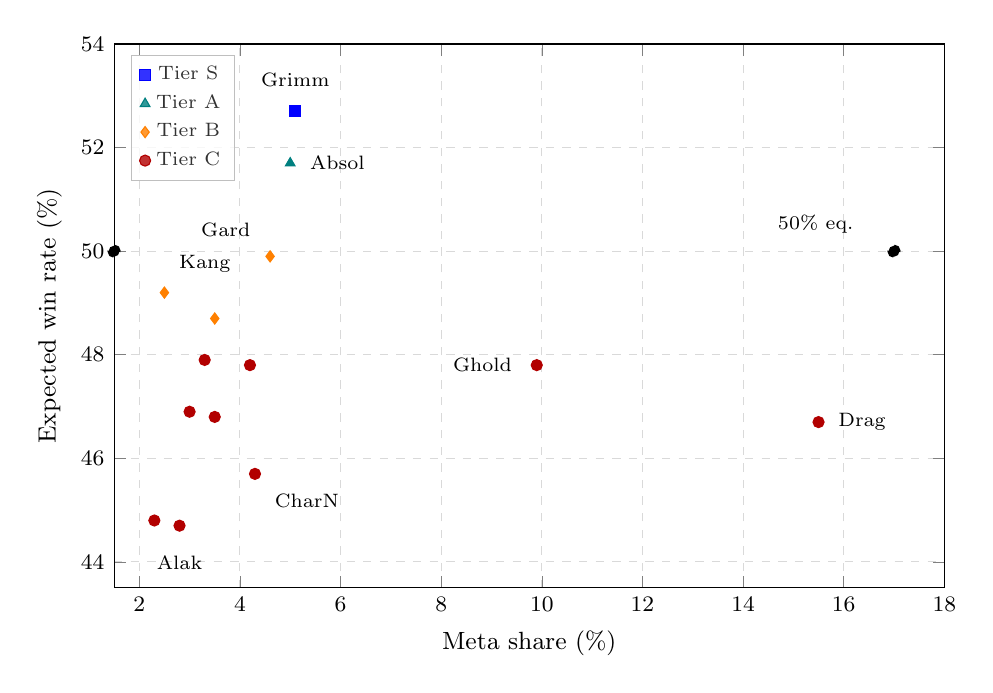
\begin{tikzpicture}
\begin{axis}[
  width=\columnwidth,
  height=0.7\columnwidth,
  xlabel={Meta share (\%)},
  ylabel={Expected win rate (\%)},
  xmin=1.5, xmax=18,
  ymin=43.5, ymax=54,
  grid=major,
  grid style={dashed, gray!30},
  every axis label/.style={font=\small},
  tick label style={font=\footnotesize},
  scatter/classes={
    S={mark=square*,blue},
    A={mark=triangle*,teal},
    B={mark=diamond*,orange},
    C={mark=*,red!70!black}
  },
  scatter, only marks,
  scatter src=explicit symbolic,
  legend style={font=\scriptsize, at={(0.02,0.98)}, anchor=north west,
                draw=gray!50, fill=white, fill opacity=0.8},
  legend entries={Tier S, Tier A, Tier B, Tier C},
  clip=false,
]
\addplot[dashed, black, thick, forget plot]
  coordinates {(1.5,50) (17,50)};
\node[font=\scriptsize, anchor=south west] at (axis cs:14.5,50.15) {50\% eq.};
\addplot[scatter, only marks, scatter src=explicit symbolic]
  coordinates { (5.1,52.7) [S] };
\addplot[scatter, only marks, scatter src=explicit symbolic]
  coordinates { (5.0,51.7) [A] };
\addplot[scatter, only marks, scatter src=explicit symbolic]
  coordinates { (4.6,49.9) [B] (3.5,48.7) [B] (2.5,49.2) [B] };
\addplot[scatter, only marks, scatter src=explicit symbolic]
  coordinates {
    (15.5,46.7) [C] (9.9,47.8) [C] (4.3,45.7) [C]
    (4.2,47.8) [C] (3.5,46.8) [C] (3.3,47.9) [C]
    (3.0,46.9) [C] (2.8,44.7) [C] (2.3,44.8) [C]
  };
\node[font=\scriptsize, anchor=west]  at (axis cs:15.7,46.7)  {Drag};
\node[font=\scriptsize, anchor=south] at (axis cs:5.1,53.0)   {Grimm};
\node[font=\scriptsize, anchor=west]  at (axis cs:5.2,51.7)   {Absol};
\node[font=\scriptsize, anchor=east]  at (axis cs:9.6,47.8)   {Ghold};
\node[font=\scriptsize, anchor=south east]  at (axis cs:4.4,50.1)   {Gard};
\node[font=\scriptsize, anchor=north west] at (axis cs:4.5,45.5)   {CharN};
\node[font=\scriptsize, anchor=north]  at (axis cs:2.8,44.3)   {Alak};
\node[font=\scriptsize, anchor=south west]  at (axis cs:2.6,49.4)   {Kang};
\end{axis}
\end{tikzpicture}
\caption{Popularity paradox: share versus expected win rate (top-14 normalized). Dragapult is high-share/low-fitness; Grimmsnarl is low-share/high-fitness.}
\label{fig:paradoxscatter}
\end{figure}

The paradox is a distributed effect: Gholdengo (9.9\% share, 43.6\% Drag WR), Gardevoir (4.6\%, 34.3\%), Grimmsnarl (5.1\%, 38.6\%), and Mega Absol (5.0\%, 38.2\%) jointly drive Dragapult's underperformance.
Dragapult's strongest offsetting lane is Charizard Noctowl (64.1\%), but that lane alone is not enough once weighted against the rest of the field.
No single catastrophic matchup is responsible, making the effect both strategically important and behaviorally persistent---it is a distributed consequence of several moderately bad, nontrivially prevalent opponents.

\subsection{Behavioral-Economic Interpretation}

The divergence between observed shares and equilibrium play is consistent with bounded-rationality explanations from behavioral game theory~\cite{Tversky1974,Kahneman1979,Banerjee1992,Bikhchandani1992,mckelvey1995quantal,nagel1995unraveling}, including familiarity bias, social diffusion, and card-access constraints.
We do not claim causal identification of these mechanisms in this dataset window; rather, we formally prove payoff-model suboptimality and treat behavioral explanations as scope-limited hypotheses for future player-level study.
This separation between proven payoff statements and behavioral interpretation disciplines narrative overreach and motivates the equilibrium/dynamics analysis in Section~\ref{sec:nash}.

%======================================================================
\section{Nash Equilibrium and Metagame Dynamics}\label{sec:nash}
%======================================================================

We model deck choice as a finite two-player bimatrix game induced by the 14$\times$14 payoff matrix~\cite{NisanRoughgarden2007}.
Existence of Nash equilibria is guaranteed by Nash's theorem~\cite{nash1950equilibrium}; von Neumann's minimax theorem applies to the zero-sum special case~\cite{vonneumann1928theorie}.
The empirical matrix is approximately constant-sum (deviations arise from the tie convention); verification uses saddle-point conditions checked for both players independently, which does not require the zero-sum assumption.
Candidate equilibrium weights were obtained via Python's \texttt{scipy.optimize.linprog}; Lean independently verifies best-response conditions for all 14 pure strategies, so the discovery tool is untrusted.

This two-player view approximates head-to-head tournament matches but does not capture Swiss-system incentives, where consistency may outweigh expected value~\cite{glickman1999parameter,herbrich2007trueskill}.
Under a risk-averse Swiss objective (maximizing probability of reaching X-2 or better), equilibrium weight shifts toward decks with consistent, if modest, win rates.
We treat this as a modeling limitation: the analysis below targets a single-match competitive benchmark, not a full Swiss-utility optimum.

\begin{lstlisting}
-- NashEquilibrium.lean
theorem real_nash_equilibrium_verified :
    NashEquilibrium realMetaGame14 realNashRow realNashCol := by
  native_decide
\end{lstlisting}

The row player's guaranteed expected payoff is ${\approx}479.7$\textperthousand{} (48.0\%), sub-50\% due to the tie convention.
Win rates are encoded on a 0--1000 scale, so a value of 479.67 corresponds to a 47.97\% win probability.
Table~\ref{tab:nash} reports the verified supports; row and column supports differ because the empirical matrix is not perfectly antisymmetric ($M_{ij} + M_{ji} \neq 1000$ for many pairs).
In a bimatrix game with approximately-constant-sum but not exactly constant-sum structure, distinct row and column supports are mathematically expected rather than anomalous.

\begin{table}[!t]
\centering
\caption{Lean-verified Nash supports for row and column strategies.}
\label{tab:nash}
\scriptsize
\begin{tabular}{@{}rlrr@{}}
\toprule
\textbf{Idx} & \textbf{Deck} & \textbf{Row wt.} & \textbf{Col wt.} \\
\midrule
1 & Gholdengo Lunatone & 0.0\% & 3.7\% \\
2 & Grimmsnarl Froslass & 37.8\% & 40.5\% \\
3 & Mega Absol Box & 12.9\% & 7.2\% \\
4 & Gardevoir & 3.5\% & 7.6\% \\
5 & Charizard Noctowl & 11.3\% & 5.0\% \\
9 & Raging Bolt Ogerpon & 28.7\% & 35.9\% \\
11 & Alakazam Dudunsparce & 5.8\% & 0.0\% \\
\bottomrule
\end{tabular}
\end{table}

We also verify a symmetric Nash equilibrium on the constant-sum symmetrization $S_{ij} = (M_{ij} + 1000 - M_{ji})/2$ (Table~\ref{tab:symmetric}), with game value exactly 500.

\begin{lstlisting}[caption={Symmetric Nash verification.},label={lst:symnash}]
theorem sym_nash_equilibrium_verified :
  NashEquilibrium symMetaGame
    symNashStrategy symNashStrategy
    := by native_decide
\end{lstlisting}

\begin{table}[!htbp]
\caption{Symmetric Nash equilibrium on the constant-sum symmetrization. Exhaustive enumeration confirms uniqueness; Dragapult is excluded with gap $-$63.3\textperthousand.}
\label{tab:symmetric}
\centering
\footnotesize
\begin{tabular}{@{}lrr@{}}
\hline
\textbf{Archetype} & \textbf{Wt.\ (\%)} & \textbf{Gap$^\dagger$} \\
\hline
Grimmsnarl       & 34.3 & 0.0 \\
Raging Bolt      & 29.4 & 0.0 \\
Charizard        & 10.2 & 0.0 \\
Mega Absol       & 10.2 & 0.0 \\
Gholdengo        &  9.2 & 0.0 \\
Gardevoir        &  4.3 & 0.0 \\
Alakazam         &  2.5 & 0.0 \\
\hline
Gard.\ Jellicent &  0.0 & $-$7.9 \\
Char.\ Pidgeot   &  0.0 & $-$13.1 \\
Kangaskhan       &  0.0 & $-$53.2 \\
\textbf{Dragapult}& \textbf{0.0} & $\mathbf{-63.3}$ \\
Drag.\ Charizard &  0.0 & $-$67.1 \\
Ceruledge        &  0.0 & $-$68.1 \\
N's Zoroark      &  0.0 & $-$71.1 \\
\hline
\multicolumn{3}{@{}l}{\scriptsize $^\dagger$Payoff gap vs.\ NE value (\textperthousand).}
\end{tabular}
\end{table}

Crucially, Dragapult (15.5\% observed share) has 0\% weight in both equilibria and is strictly suboptimal against the Nash column mix (\texttt{dragapult\_strictly\_suboptimal}).

\paragraph{Uniqueness of the symmetric equilibrium}
Exhaustive support enumeration over all $2^{14} - 1 = 16{,}383$ subsets confirms the constant-sum symmetrization admits exactly one symmetric Nash equilibrium.
Of the 8{,}192 subsets containing Dragapult, none yields a valid equilibrium.
Dragapult's payoff against the equilibrium mix is 416.7\textperthousand, a gap of 63.3 below the equilibrium value, confirming it is strictly dominated by the equilibrium mixture.
The equilibrium is non-degenerate (exactly five best responses matching support size), implying uniqueness by the non-degeneracy theorem for constant-sum games.
This upgrades the existential claim (``there exists an equilibrium excluding Dragapult'') to a universal one: no symmetric Nash equilibrium assigns Dragapult positive weight.
Combined with the sensitivity analysis (77.9\% Dragapult exclusion across 10{,}000 resampled matrices), this provides strong evidence that observed popularity can lie entirely outside equilibrium support.

\subsection{Replicator Dynamics}

Replicator dynamics formalize directional pressure~\cite{Hofbauer1998,Sandholm2010}:
$\dot{x}_i = x_i(f_i(\mathbf{x}) - \bar{f}(\mathbf{x}))$.
Our Lean implementation uses discrete-time Euler steps; all verified results are single-step directional statements from the observed share vector.

\begin{lstlisting}
-- Full 14-deck replicator dynamics
theorem full_replicator_dragapult_decline :
    fitness 14 fullPayoff fullMeta ⟨0, ..⟩ < avgFitness 14 fullPayoff fullMeta := by
  native_decide
theorem full_replicator_grimmsnarl_fittest :
    ∀ i, fitness 14 fullPayoff fullMeta i ≤
         fitness 14 fullPayoff fullMeta ⟨5, ..⟩ := by
  native_decide
\end{lstlisting}

The full classification identifies 5 growing and 9 shrinking archetypes:
(i)~Dragapult has below-average fitness and should lose share,
(ii)~Grimmsnarl has the highest fitness among all 14 archetypes, and
(iii)~Alakazam faces the strongest extinction pressure.
The directional classification is algebraically step-size-independent: since $x_i' - x_i = x_i \cdot \mathrm{dt} \cdot (f_i - \bar{f})$, the sign depends only on $f_i - \bar{f}$, not on $\mathrm{dt}$; this is proved as a general kernel-level lemma (\texttt{rat\_replicator\_sign\_independent\_of\_dt}) using \texttt{simp}, \texttt{ring}, and \texttt{omega}---without \texttt{native\_decide}.
Concrete verification at $\mathrm{dt} = 1/10$, $1/100$, and $1$ (\texttt{StepSizeInvariance.lean}) confirms the identical 5-grower/9-shrinker partition in all cases.

A discrete replicator step confirms that Grimmsnarl's share increases while Dragapult's decreases (\texttt{grimmsnarl\_share\_increases}, \texttt{dragapult\_share\_decreases}).

\begin{figure}[!t]
\centering
\[
\begin{array}{ccc}
\text{Raging Bolt} & \xrightarrow{67.3\%} & \text{Mega Absol} \\
\downarrow_{51.0\%} & & \downarrow_{62.1\%} \\
\text{Dragapult} & \xleftarrow{57.2\%} & \text{Grimmsnarl}
\end{array}
\]
\caption{Directed metagame interaction motif.}
\label{fig:cycle}
\end{figure}

Figure~\ref{fig:cycle} emphasizes that the ecosystem is interaction-rich rather than strictly ordered, explaining persistent diversity even though the verified Nash support has only six decks.
We therefore treat replicator outputs as directional diagnostics: Dragapult pressure is downward, Grimmsnarl pressure is upward, and Alakazam pressure is extinction-like.
These directions are falsifiable against subsequent tournament windows and provide a compact bridge from static equilibrium objects to week-to-week metagame interpretation.

\subsection{Preliminary Directional Check}

As a preliminary predictive check, two of three directional predictions were confirmed against Trainer Hill trend data one day after the analysis window: Mega Absol and Gardevoir both showed upward trending as predicted.
However, Grimmsnarl showed downward trending despite highest fitness---a secondary effect of Mega Absol's rise creating predation pressure on Grimmsnarl (Mega Absol beats Grimmsnarl 61.4\%).
This multi-step cascade illustrates a limitation of single-step replicator analysis: even with the full 14-deck model, one-step predictions do not capture iterated dynamics where a rising counter-deck suppresses its prey.
Iterated replicator simulation over many steps would be needed for accurate multi-step trajectory predictions.

%======================================================================
\section{Tournament Strategy}\label{sec:tournament}
%======================================================================

Most major events run best-of-three (Bo3) matches and Swiss-style pairings.
For game win probability $p$, Bo3 match win probability is $P_{\mathrm{Bo3}} = 3p^2 - 2p^3$.
The Pok\'emon TCG lacks sideboarding, making the independence assumption more defensible than in other TCGs; however, tilt effects and information revelation (observing the opponent's deck in game one) introduce minor dependencies that our model does not capture.
Lean verifies that Bo3 amplifies advantage for all favorable rates from 55\% to 95\% (\texttt{BO3\_AMPLIFIES\_ADVANTAGE}).
The Bo3 formula is cubic and monotonically amplifying:
for $p > 0.5$, $P_{\mathrm{Bo3}}(p) > p$, and the amplification $P_{\mathrm{Bo3}} - p$ increases with $p$, reaching its maximum at $p = 0.75$ where a single-game 75\% edge becomes an 84.4\% match advantage.
This non-linearity means that even moderate matchup edges become strategically dominant in match play.
Table~\ref{tab:bo3} shows that large single-game edges become very hard to overcome in match play.

\begin{table}[!t]
\centering
\caption{Bo1 to Bo3 Amplification for Key Matchups.}
\label{tab:bo3}
\begin{tabular}{lcc}
\toprule
\textbf{Matchup} & \textbf{Bo1} & \textbf{Bo3} \\
\midrule
Raging Bolt vs Mega Absol & 67.3\% & 74.9\% \\
Gardevoir vs Dragapult & 62.7\% & 68.6\% \\
Mega Absol vs Grimmsnarl & 62.1\% & 67.8\% \\
Grimmsnarl vs Dragapult & 57.2\% & 60.7\% \\
Dragapult vs Charizard Noctowl & 64.1\% & 70.6\% \\
\bottomrule
\end{tabular}
\end{table}

Table~\ref{tab:bo3} shows that large single-game edges become very hard to overcome in match play, increasing the value of targeted counter slots.

Swiss tournaments further reward consistency: for an eight-round event with an X--2 qualification target and field-level Bo3 win probability $p_m$, the cut-line probability is
$P(\text{X--2 or better}) = \sum_{k=6}^{8} \binom{8}{k} p_m^k (1-p_m)^{8-k}$.
Registration should combine projected field shares, weighted expected WR, and stress tests on the largest counter-edges rather than rely on average EV alone.

%======================================================================
\section{Formalization Methodology}\label{sec:methodology}
%======================================================================

The development enforces a strict \textbf{zero-axiom, zero-sorry standard}: no \texttt{sorry}, no \texttt{admit}, and no custom axioms, turning persuasive-but-brittle metagame narratives into inspectable, machine-checked artifacts.
The artifact comprises 81 files and approximately 30{,}200 lines across seven module groups, totaling over 2{,}500 theorems of which ${\sim}$190 directly verify empirical claims, including 12 end-to-end cross-module integration theorems (\texttt{IntegrationTests.lean}).

Most proofs follow one of four patterns:
(1)~decision procedures over finite domains (\texttt{native\_decide}, \texttt{decide}),
(2)~arithmetic normalization (\texttt{omega}, \texttt{nlinarith}),
(3)~definitional unfolding and rewriting (\texttt{simp}), and
(4)~decomposition of strategic statements into finite conjunctions over concrete decks.

\subsection{Trust Boundary: \texttt{native\_decide}}\label{subsec:trust}

All computational proofs use \texttt{native\_decide}, which compiles decidability witnesses to native code and trusts Lean's compiler rather than its kernel.
Of the ${\sim}$2{,}500 theorems, roughly 244 use \texttt{native\_decide} directly (including all Nash equilibrium, replicator dynamics, and bridge alignment theorems); the remainder close via \texttt{decide}, \texttt{simp}, \texttt{omega}, or structural tactics.
Table~\ref{tab:assurance} summarizes assurance levels.

\begin{table}[!t]
\centering
\caption{Assurance levels by theorem category. \emph{Kernel} = fully checked by Lean's trusted kernel; \emph{Compiler} = trusts native code generation.}
\label{tab:assurance}
\footnotesize
\begin{tabular}{@{}lccl@{}}
\toprule
\textbf{Category} & \textbf{Count} & \textbf{Level} & \textbf{Tactics} \\
\midrule
Rules \& legality        & 180  & Kernel   & \texttt{decide}, \texttt{simp} \\
Card effects             & 120  & Kernel   & \texttt{simp}, \texttt{omega} \\
Probability              & 90   & Kernel   & \texttt{decide}, \texttt{omega} \\
Step-size invariance     & 4    & Kernel   & \texttt{simp}, \texttt{ring}, \texttt{omega} \\
Infrastructure           & 1{,}862 & Kernel & mixed \\
\midrule
Nash equilibrium         & 12   & Compiler & \texttt{native\_decide} \\
Replicator dynamics      & 38   & Compiler & \texttt{native\_decide} \\
Bridge alignment (type)  & 25   & Compiler & \texttt{native\_decide} \\
Sensitivity / robustness & 42   & Compiler & \texttt{native\_decide} \\
Other matrix computations& 127  & Compiler & \texttt{native\_decide} \\
\midrule
\textbf{Total}           & \textbf{2{,}500} & & \\
\bottomrule
\end{tabular}
\end{table}

We investigated replacing \texttt{native\_decide} with the kernel-checked \texttt{decide}, but it is \emph{structurally precluded}: our matrix computations use \texttt{Fin.foldl}, which is opaque to the Lean~4 kernel reducer.
This is a known limitation of the current kernel, not specific to our proofs.
The trust implications are worth stating explicitly: \texttt{native\_decide} does not produce a proof term that the kernel independently verifies, and a hypothetical bug in Lean~4's code generator affecting rational arithmetic over \texttt{Fin.foldl} could simultaneously invalidate all 244 \texttt{native\_decide} proofs.
We note that no such bugs have been reported in practice, and \texttt{native\_decide} is the standard approach for computational proofs over finite structures in the Lean community~\cite{moura2021lean}.
A kernel-transparent reimplementation or future kernel improvements would enable fully kernel-checked verification.

\subsection{Reproducibility and Cost-Benefit}

Every statistic used for strategic claims can be traced to an explicit Lean constant and theorem, and every theorem is checkable by rebuilding the project with the published sources.
Data tables match constants in \texttt{RealMetagame.lean} and \texttt{MatchupAnalysis.lean}; key strategic claims are mirrored by named theorems.
This one-to-one mapping sharply reduces the risk of drift between code and prose.
A cross-file consistency theorem (\texttt{MatrixConsistency.lean}) machine-checks that array-based and function-based matrix representations agree, eliminating a class of copy-paste errors across module boundaries.
A Python script can recompute percentages quickly, but it does not enforce theorem-level linkage between assumptions, constants, and manuscript claims.
The Lean pipeline adds that linkage and fails loudly when any claim drifts from its formal source.

Updating the analysis for a new tournament window requires changing only \texttt{RealMetagame.lean} (${\sim}$200 lines); all downstream theorems either re-verify automatically or fail with precise error locations.
The fixed cost is high but the marginal cost of validated updates is low.
During development, the best-response certification failed several times due to data-entry errors in the 14$\times$14 matchup matrix (swapped row/column indices, copy-paste duplication of a row).
Each failure was caught immediately by \texttt{native\_decide} returning \texttt{false}, pinpointing the exact cell---errors that Python's \texttt{scipy.optimize.linprog} would have silently absorbed, since the LP solver treats any matrix as valid.

\begin{table}[!t]
\centering
\caption{Methodology comparison for metagame analytics.}
\label{tab:baseline}
\footnotesize
\begin{tabular}{@{}lccc@{}}
\toprule
\textbf{Method} & \textbf{LoC} & \textbf{Runtime} & \textbf{Guarantee} \\
\midrule
Spreadsheet     & $\sim$50 cells & minutes & manual review \\
Python + scipy  & $\sim$100      & $<$1\,s & unit tests \\
Lean~4 (ours)   & $\sim$30K      & $\sim$10\,min & verified$^*$ \\
\bottomrule
\multicolumn{4}{@{}l}{\scriptsize $^*$Modulo \texttt{native\_decide}; see Section~\ref{sec:methodology}.}
\end{tabular}
\end{table}

The apparent LOC-to-insight ratio (30K lines for conclusions derivable from a spreadsheet) is misleading: the ``excess'' code is infrastructure that enables compositional reuse.
The fixed cost is high but the marginal cost of validated updates is low.

\subsection{Case Study: Verifying a Headline Claim}

To illustrate traceability, consider ``Dragapult is 15.5\% of the meta but only 46.7\% expected.'' This decomposes into six auditable steps: extract shares from Trainer Hill data, normalize to the top-14 subfield, compute weighted expectation $\sum_j s_j w_{i,j}$, express as exact rational in Lean, prove the inequality $\mathbb{E}[\mathrm{WR}_{\mathrm{Drag}}] < 500$, and reuse constants in tables.
If any upstream value changes, downstream theorems fail, making drift explicit---fundamentally stronger than spreadsheet pipelines where hidden references silently desynchronize.

\subsection{Human Review and Artifact Audit}

Human review remains essential for model scope.
Our audit checks (i)~data fidelity to source snapshots, (ii)~theorem statement correctness relative to intended claims, and (iii)~narrative discipline---no prose claim without formal or computed backing.
This lightweight process catches copy-edit drift, stale entries, and implicit assumptions that escape the type checker.

%======================================================================
\section{Threats to Validity}\label{sec:threats}
%======================================================================

\textbf{Temporal locality.}
The analyzed window is three weeks; metagames shift rapidly due to innovation, counter-adaptation, and card availability.
Our claims describe this window precisely; they are not universal constants.
However, temporal locality is not purely a weakness: short windows reduce hidden confounding from major ruleset changes.
Future work should combine rolling windows with change-point detection to separate genuine adaptation from transient noise.

\textbf{Top-14 normalization.}
Expected win rates are normalized over the modeled 69.5\% top-14 subset.
Machine-checked worst-case bounds show that Dragapult requires at least 57.6\% win rate against all unmodeled archetypes merely to reach 50\% overall---well above the coin-flip baseline---while Grimmsnarl remains above 50\% unless its unmodeled win rate drops below 43.9\%.
Share-perturbation theorems (\texttt{SharePerturbation.lean}) confirm the paradox is structural: even with Dragapult's share at 5\%, its expected WR remains below 50\%; conversely, if Grimmsnarl's share rises to 15.5\%, its expected WR remains above 50\%.
The paradox derives from the matchup matrix, not the share vector.

\textbf{Archetype granularity.}
Each archetype is treated as a point strategy; list-level technology choices and pilot skill heterogeneity introduce within-archetype variance not captured by the matrix.
This is a standard abstraction tradeoff: coarse archetype bins improve statistical power but hide intra-bin adaptation.
A natural extension is hierarchical modeling with sub-archetype clusters once sample sizes permit.

\textbf{Player-skill confounding.}
Matchup win rates aggregate across all skill levels.
If popular archetypes attract less experienced pilots, their observed win rates may be suppressed by player-quality effects rather than deck-strength effects.
Machine-checked sensitivity bounds (\texttt{SkillSensitivity.lean}) show Dragapult would need a uniform skill-bias correction of at least 3.4pp across \emph{all} matchups to reach 50\% expected WR, and 6.1pp to match Grimmsnarl---implying a confound large enough to reverse the paradox would require implausibly large, uniform skill deficits among Dragapult pilots.
Based on competitive experience and available tournament analytics, within-event skill differentials in large TCG events are unlikely to exceed 5pp uniformly across all matchups; the 6.1pp Grimmsnarl-matching threshold exceeds any plausible uniform confound.

\textbf{Strategic objective mismatch.}
Players optimize mixed objectives (comfort, risk tolerance, card access); observed non-equilibrium play can be rational under private utility functions.
Our ``suboptimal'' terminology is relative to the stated payoff model.

With these limitations explicit, we summarize the main findings and concrete next steps.

%======================================================================
\section{Conclusion}\label{sec:conclusion}
%======================================================================

This paper presents a metagame analysis pipeline for a real competitive TCG, verified modulo the \texttt{native\_decide} trust boundary (Section~\ref{sec:methodology}) in Lean~4.
Using Trainer Hill data, we prove a popularity paradox (Dragapult at 15.5\% share has 46.7\% expected WR; Grimmsnarl at 5.1\% share leads with 52.7\%), connect it to a Lean-verified Nash equilibrium with 0\% Dragapult weight (unique across all $2^{14}-1$ symmetric support subsets), and show via full 14-deck replicator dynamics that Dragapult faces downward fitness pressure while Grimmsnarl has the highest fitness.
Bo3 amplification further widens key matchup edges (67.3\%\,$\to$\,74.9\%).
The specific metagame results are illustrative of the methodology, which is the primary contribution: we demonstrate that formal methods can serve as a practical scientific instrument for competitive game ecosystems.

Immediate next steps: (i)~rolling weekly windows with uncertainty intervals for forecast calibration, (ii)~explicit modeling of the 30.5\% ``Other'' segment, and (iii)~hierarchical sub-archetype clustering to capture list-level variance and pilot heterogeneity.
Our current encoding represents win rates as natural numbers on a 0--1000 scale; a richer encoding carrying individual game outcomes would enable in-Lean confidence interval computation and sample-size adequacy checks.
A natural extension would embed the sensitivity analysis within Lean using verified interval arithmetic over the linear program, eliminating the Python dependency entirely.
While Lean~4's \texttt{Mathlib} provides foundations for interval arithmetic, the LP solver integration remains an engineering challenge we leave to future work.

\subsection{Broader Implications}

This case study suggests a general template: formalize core mechanics, encode empirical payoffs as exact values, express strategic claims as theorems, and tie them to tournament objectives.
The pipeline is portable to any domain with discrete strategies and measurable outcomes.
Proof-assisted workflows do not replace domain expertise; they structure it, making conclusions machine-auditable rather than rhetorical.
Formal artifacts can serve as verified baselines for testing teams, and our results show that proof assistants are practical for empirical strategic science when domains provide structured, finite data.

\section*{Data Availability}
Data were extracted from Trainer Hill (trainerhill.com) on February~19, 2026, for events with $\geq$50 players (January~29--February~19, 2026).
The full 14$\times$14 matchup matrix, all Lean~4 source, and build instructions are included as supplementary material; reviewers can verify all claims via \texttt{lake build} (${\sim}$10\,min on Apple M-series, 16\,GB RAM).

% Balance final columns naturally.
\IEEEtriggeratref{28}
\bibliographystyle{IEEEtran}
\bibliography{references}

\end{document}
